\documentclass{standalone}
\usepackage{tikz}
\usepackage{adjustbox}
\usepackage{helvet}  
\usepackage{sansmathfonts}  
\renewcommand{\familydefault}{\sfdefault}  
\usetikzlibrary{arrows.meta,calc,decorations.pathmorphing}
\usetikzlibrary{shapes.geometric, shapes.arrows}
\usepackage{xcolor}


\begin{document}
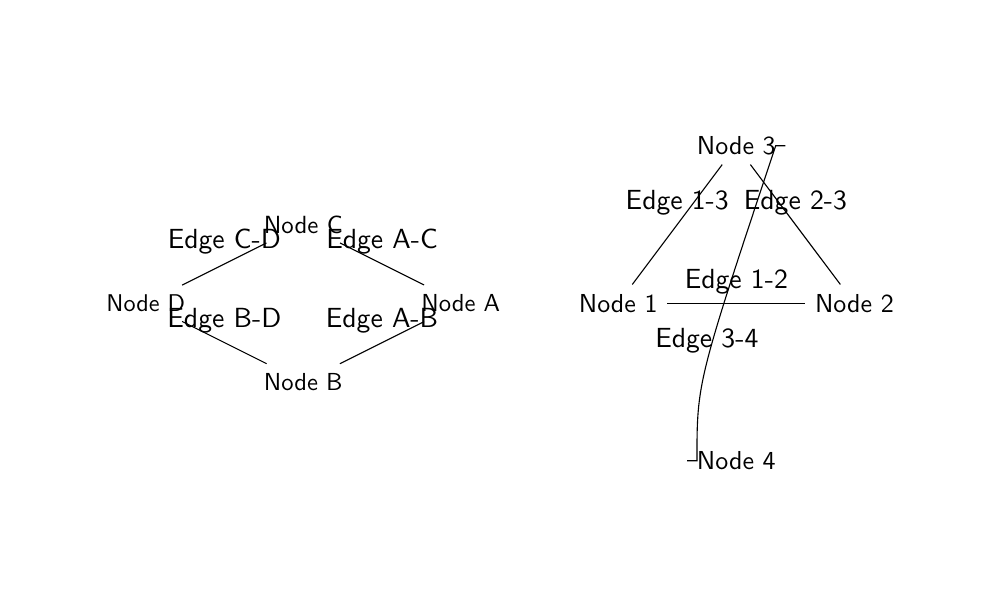
\begin{tikzpicture}
\useasboundingbox (-7.5,-3.5) rectangle (4.5,3.5);



\node[] (node1) at (0,0) {\adjustbox{max width=1cm, max height=1cm}{Node 1}};
\node[] (node2) at (3,0) {\adjustbox{max width=1cm, max height=1cm}{Node 2}};
\node[] (node3) at (1.5,2) {\adjustbox{max width=1cm, max height=1cm}{Node 3}};
\node[] (node4) at (1.5,-2) {\adjustbox{max width=1cm, max height=1cm}{Node 4}};
\node[] (nodeA) at (-2,0) {\adjustbox{max width=1cm, max height=1cm}{Node A}};
\node[] (nodeB) at (-4,-1) {\adjustbox{max width=1cm, max height=1cm}{Node B}};
\node[] (nodeC) at (-4,1) {\adjustbox{max width=1cm, max height=1cm}{Node C}};
\node[] (nodeD) at (-6,0) {\adjustbox{max width=1cm, max height=1cm}{Node D}};
\draw[] (node1) (node1) to node[above] {Edge 1-2} (node2);
\draw[] (node1) -- (node3) node[above, pos=0.5] {Edge 1-3};
\draw[] (node2) (node2) to node[above] {Edge 2-3} (node3);
\draw[] (node3) -- (2,2) .. controls (1,-1) .. (1,-2) node[above, pos=0.5] {Edge 3-4} -- (node4);
\draw[] (nodeA) (nodeA) to node[above] {Edge A-B} (nodeB);
\draw[] (nodeA) -- (nodeC) node[above, pos=0.5] {Edge A-C};
\draw[] (nodeB) (nodeB) to node[above] {Edge B-D} (nodeD);
\draw[] (nodeC) (nodeC) to node[above] {Edge C-D} (nodeD);

\end{tikzpicture}
\end{document}